\documentclass[12pt,a4paper]{paper}
\usepackage[brazil]{babel}
\usepackage[T1]{fontenc}
\usepackage[utf8]{inputenc}
\usepackage[letterpaper,top=2cm,bottom=2cm,left=2cm,right=2cm,marginparwidth=1.75cm]{geometry}

\usepackage{amsmath}
\usepackage{graphicx}
\usepackage{cite}
\usepackage[hidelinks]{hyperref}
\usepackage[printonlyused]{acronym}
\usepackage{microtype}

\usepackage{booktabs}
\usepackage{tabularx}
\usepackage{array}

\newcolumntype{L}[1]{>{\raggedright\arraybackslash}p{#1}}
\newcolumntype{Y}{>{\raggedright\arraybackslash}X}

\usepackage{multirow}
\usepackage{longtable}

\usepackage{indentfirst}
\setlength{\parindent}{0.5cm}

\usepackage{tikz}
\usetikzlibrary{arrows.meta, positioning, calc}

\usepackage{siunitx}

\usepackage{import}

\title{RSSF para Monitoramento Ambiental}
\author{Matheus Renó Torres}
\date{}

\begin{document}
\maketitle

% \begin{abstract}

% \end{abstract}

%\textbf{Palavras-chave:} 

\acrodef{RSSF}{Rede de Sensores Sem Fio}

\section{Introdução}
\label{sec:introducao}

O monitoramento ambiental por \ac{RSSF} permite a medição contínua e distribuída de variáveis relacionadas ao microclima, à qualidade do ar, às condições do solo, à qualidade da água e à ocorrência de eventos naturais \cite{HART2006177}.
Para viabilizar essa observação, uma aplicação de \ac{RSSF} para monitoramento ambiental consiste em uma rede distribuída de nós sensores que realizam medições \textit{in situ} e encaminham os dados, por enlaces sem fio, a um nó sorvedouro ou gateway, que os disponibiliza a um servidor de armazenamento e processamento \cite{5597912,AKYILDIZ2002393}.

Essa configuração reduz a necessidade de cabeamento de comunicação, facilita a instalação de múltiplos pontos de medição e possibilita observações de longa duração em áreas extensas, remotas ou de difícil acesso \cite{HART2006177,5597912}.
Como resultado, uma das principais vantagens das \acp{RSSF} no monitoramento ambiental é combinar elevada resolução espacial, mediante medições em múltiplos locais, com elevada resolução temporal, obtida por amostragens repetidas e coordenadas \cite{HART2006177,5597912}.

Essa capacidade foi demonstrada em implantações clássicas em habitats naturais, nas quais uma \ac{RSSF} registrou temperatura, umidade, pressão atmosférica e luminosidade, reduzindo a necessidade de visitas frequentes e a consequente perturbação do local \cite{10.1145/570738.570751}.
Para que os registros resultantes tenham utilidade científica, devem ser consideradas a qualidade das medições, a consistência das marcas temporais, a localização dos nós, a continuidade das séries e a confiabilidade da transmissão \cite{5597912,YICK20082292,10.1145/1031495.1031521}.
\section{Arquitetura do Sistema}

Para fins de implementação, a arquitetura pode ser organizada em quatro níveis funcionais: sensores, nós de aquisição, gateway e plataforma de dados \cite{5597912,AKYILDIZ2002393}.
Com base nessa organização, os nós realizam a amostragem das variáveis ambientais, associam identificadores e marcas temporais aos dados, executam verificações locais de consistência e encaminham os registros ao gateway \cite{YICK20082292,5597912}.
Por sua vez, o gateway agrega os pacotes recebidos dos nós sensores e os encaminha, por meio de um enlace de backhaul, a um servidor local ou remoto \cite{5597912,10.1145/570738.570751}.
Para preservar a continuidade da aquisição, o armazenamento temporário nos nós ou no gateway permite manter a coleta durante interrupções do enlace de backhaul e transmitir os registros após o restabelecimento da conexão \cite{5597912,10.1145/1031495.1031521}.

A cadeia funcional resultante é apresentada na Figura \ref{fig:arquitetura_funcional}.
Além da organização do fluxo de dados, a implantação exige atenção à autonomia energética, ao encapsulamento, à calibração e à manutenção, pois falhas nesses elementos podem produzir lacunas ou medições sem validade científica \cite{5597912,10.1145/1031495.1031521}.

\begin{figure}[!ht]
    \centering
    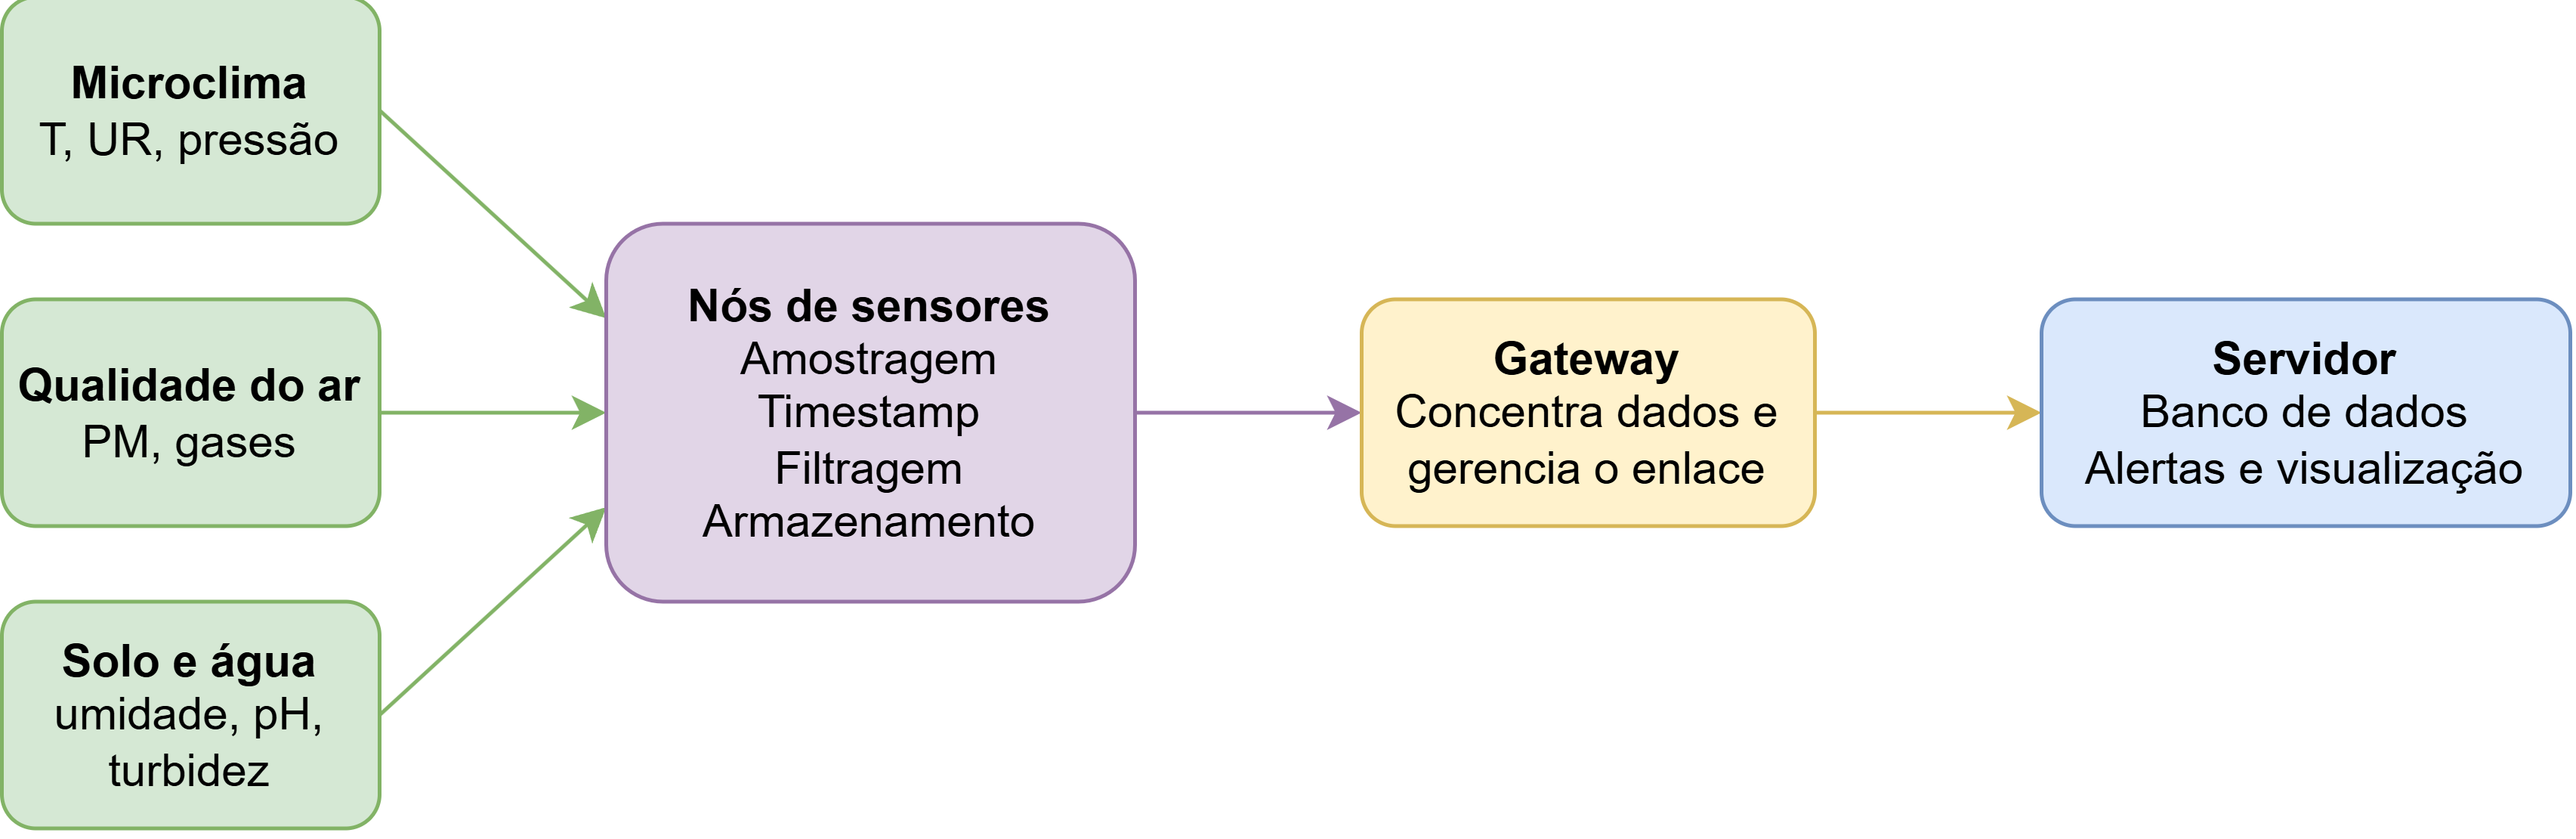
\includegraphics[width=0.98\columnwidth]{figures/arquitetura_funcional.drawio.png}
    \caption{Arquitetura funcional de uma RSSF ambiental.}
    \label{fig:arquitetura_funcional}
\end{figure}
\section{Nós e Topologia}

Cada nó sensor integra transdutores, circuitos de condicionamento e aquisição de sinais, unidade de processamento com memória, transceptor sem fio e fonte de energia \cite{AKYILDIZ2002393}.
Nessa estrutura, o microcontrolador controla o ciclo de amostragem, aplica conversões e verificações de plausibilidade, associa marcas temporais às medições e pode executar agregação ou detecção local de eventos antes do envio dos dados \cite{YICK20082292,ANASTASI2009537,5597912}.
Para reduzir a perda de dados durante indisponibilidades breves do enlace, o armazenamento temporário em memória local permite preservar as medições e encaminhá-las após o restabelecimento da comunicação, desde que a capacidade do buffer seja suficiente \cite{5597912,10.1145/1031495.1031521}.

A Figura \ref{fig:no_sensor_ambiental} sintetiza os blocos funcionais descritos.

\begin{figure}[!ht]
    \centering
    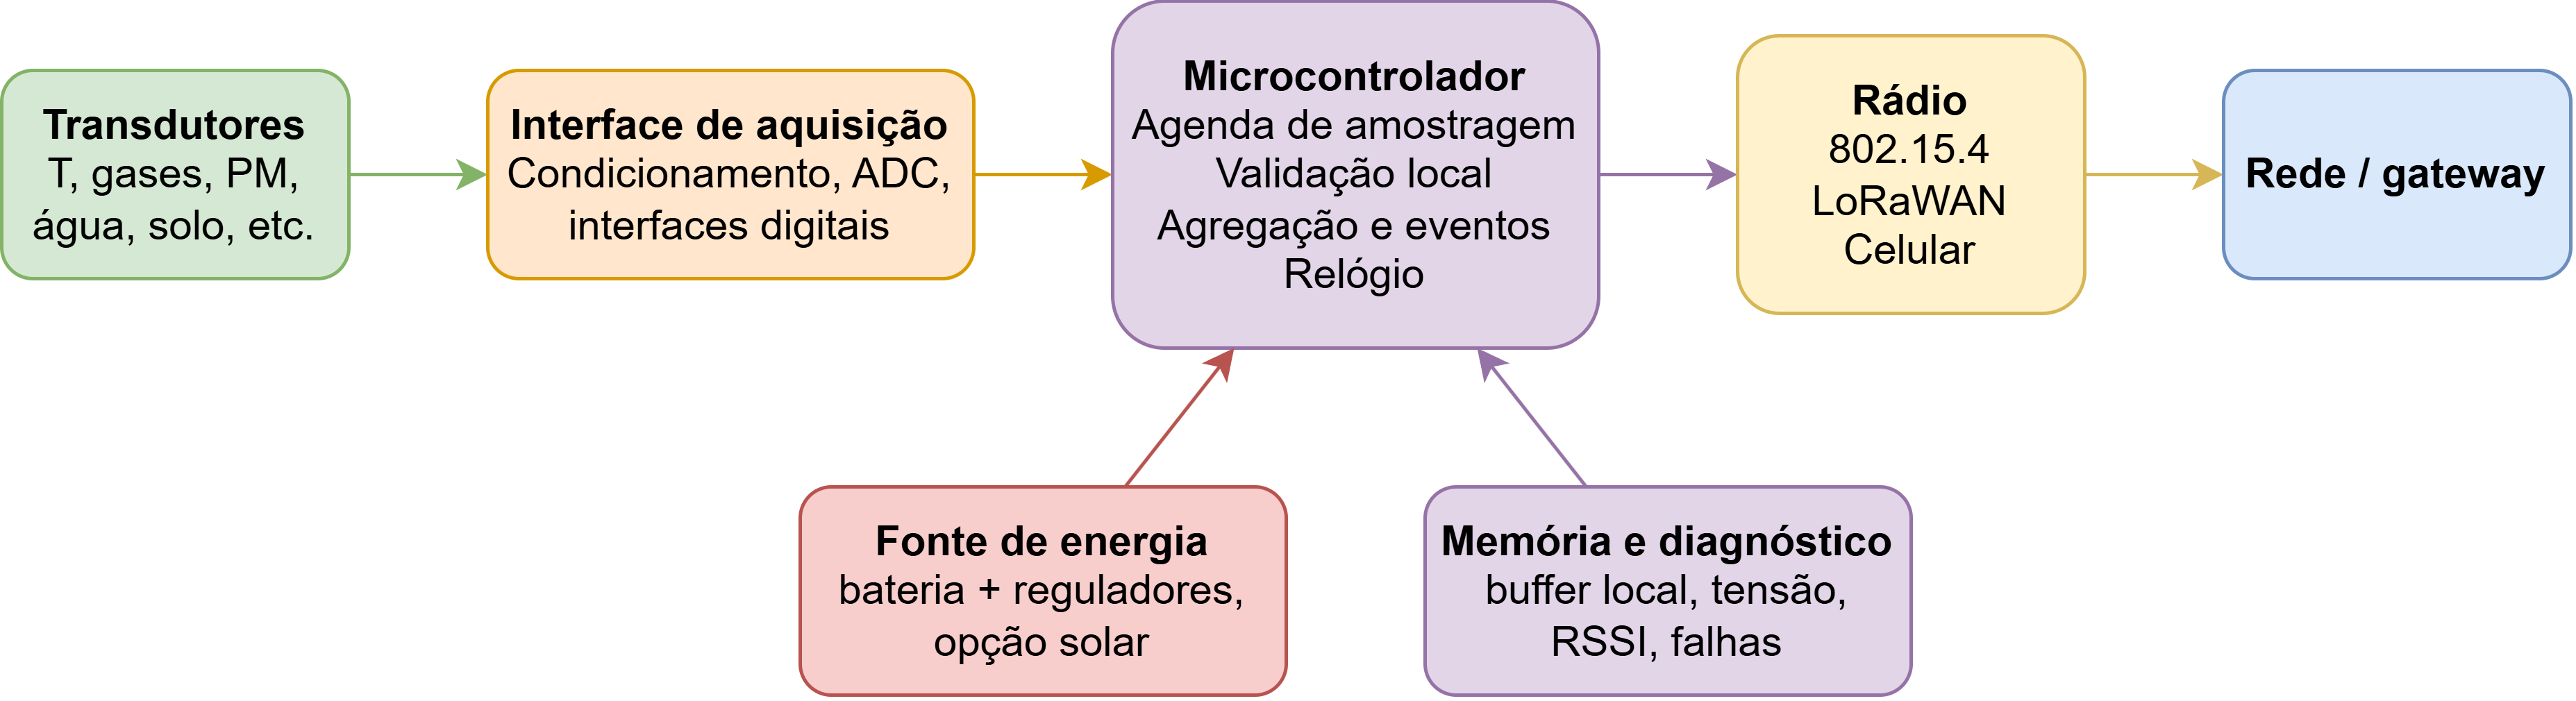
\includegraphics[width=0.98\columnwidth]{figures/blocos_funcionais_sensor_ambiental.drawio.png}
    \caption{Blocos funcionais de um nó sensor ambiental.}
    \label{fig:no_sensor_ambiental}
\end{figure}

A topologia da \ac{RSSF} é definida em função da extensão da área, do relevo, da distribuição dos pontos de medição e das condições de propagação dos enlaces \cite{10.1145/1134680.1134685,5597912}.
Quando todos os nós mantêm enlace direto com o gateway, uma topologia em estrela é adequada. Em topologias multi-hop, o encaminhamento por nós intermediários pode ampliar a cobertura em áreas com obstáculos, porém aumenta o consumo energético e faz a entrega depender da disponibilidade dos nós retransmissores \cite{YICK20082292,ANASTASI2009537,10.1145/1031495.1031521}.
Para aplicações distribuídas por áreas extensas e com baixa taxa de geração de dados, uma LPWAN pode ampliar a área atendida por cada gateway e reduzir a densidade de infraestrutura necessária \cite{7815384}.
Em qualquer dessas configurações, a seleção do protocolo de comunicação depende da análise conjunta do alcance, da taxa de dados, do consumo energético, das condições de propagação impostas pelo relevo e pela vegetação, da infraestrutura disponível e do custo \cite{5597912,7815384,8030482,10.1145/1134680.1134685}.
\section{Sensores e Calibração}

Os principais sensores estão resumidos na Tabela \ref{tab:sensores_ambientais}.
Um nó pode integrar diferentes sensores, desde que cada transdutor seja instalado de acordo com a variável medida e com suas condições de exposição. Sensores de temperatura do ar requerem abrigo ventilado e proteção contra radiação solar direta; sondas de solo exigem contato estável com o substrato; e sensores de qualidade da água requerem imersão adequada e manutenção periódica para controle da bioincrustação \cite{5597912,10.1145/3005719,s23146332}.

Quanto à qualidade metrológica, sensores de baixo custo permitem aumentar a densidade espacial do monitoramento. Sua equivalência a instrumentos de referência depende de calibração, co-localização e validação nas condições de operação \cite{atmos10090506,KANG2022151769}.
Em particular, estudos sobre sensores de baixo custo para qualidade do ar identificam a temperatura, a umidade, a deriva temporal, as sensibilidades cruzadas e o modelo de calibração como fatores que influenciam a resposta dos dispositivos \cite{atmos10090506,KANG2022151769}.
Com base nesses fatores, recomenda-se co-localizar uma parcela dos nós com um instrumento de referência, documentar o modelo e a versão da calibração aplicada e repetir a verificação durante a implantação para identificar alterações de desempenho \cite{atmos10090506,KANG2022151769}.

\begin{table*}[!t]
\centering
\caption{Variáveis, princípios de medição e requisitos de implantação para o monitoramento ambiental.}
\label{tab:sensores_ambientais}
\footnotesize
\setlength{\tabcolsep}{4pt}
\renewcommand{\arraystretch}{1.18}

\begin{tabularx}{\textwidth}{
    @{}
    L{2.0cm}
    L{3.6cm}
    Y
    Y
    @{}
}
\toprule
\textbf{Grupo} &
\textbf{Variáveis monitoradas} &
\textbf{Princípios de medição e sensores} &
\textbf{Requisitos de implantação e manutenção} \\
\midrule

Água
\cite{10.1145/3005719} &
Temperatura, pH, turbidez, oxigênio dissolvido e condutividade elétrica &
Termistor ou RTD; eletrodo de pH; turbidímetro óptico; sensor óptico ou eletroquímico de oxigênio dissolvido; célula de condutividade &
Controle de bioincrustação; compensação de temperatura; limpeza periódica; verificação e recalibração dos sensores \\

\addlinespace

Eventos naturais
\cite{10.1145/1134680.1134685} &
Nível da água, vibração do solo, pressão acústica, fumaça e velocidade do vento &
Transdutor de pressão ou sensor ultrassônico; acelerômetro ou geofone; microfone; detector óptico de fumaça; anemômetro &
Definição e validação dos limiares; sincronização temporal; aquisição disparada por evento; armazenamento temporário local \\

\addlinespace

Microclima
\cite{HART2006177,5597912,10.1145/570738.570751} &
Temperatura do ar, umidade relativa e pressão atmosférica &
Termistor, RTD ou sensor digital de temperatura; sensor capacitivo de umidade; barômetro MEMS &
Abrigo meteorológico ventilado; altura e exposição padronizadas; proteção contra radiação solar direta e condensação \\

\addlinespace

Qualidade do ar
\cite{atmos10090506,KANG2022151769} &
\(\mathrm{PM}_{2{,}5}\), \(\mathrm{PM}_{10}\), \(\mathrm{CO}_{2}\), \(\mathrm{CO}\), \(\mathrm{NO}_{2}\), \(\mathrm{O}_{3}\) e compostos orgânicos voláteis &
Contador óptico de partículas; sensor NDIR; células eletroquímicas; sensores de óxido metálico &
Co-localização com instrumento de referência; calibração; compensação de temperatura e umidade; avaliação de deriva e sensibilidade cruzada \\

\addlinespace

Radiação solar e precipitação
\cite{5597912} &
Iluminância, irradiância solar e precipitação &
Fotodiodo ou luxímetro; piranômetro; pluviômetro de báscula &
Nivelamento; campo de visão desobstruído; controle de sombreamento; limpeza e inspeção periódicas \\

\addlinespace

Solo
\cite{5597912,s23146332} &
Teor volumétrico de água, temperatura e condutividade elétrica &
Sensor capacitivo, FDR ou TDR; termistor ou RTD; eletrodos de condutividade &
Contato adequado com o solo; calibração para o tipo de solo; avaliação do efeito da salinidade; distribuição espacial representativa dos pontos \\

\bottomrule
\end{tabularx}

\vspace{3pt}
\parbox{\textwidth}{\footnotesize
RTD: detector resistivo de temperatura;
MEMS: sistemas microeletromecânicos;
NDIR: infravermelho não dispersivo;
FDR: reflectometria no domínio da frequência;
TDR: reflectometria no domínio do tempo.
}
\end{table*}
\section{Tecnologias de Comunicação}

A seleção da tecnologia de comunicação deve considerar o tamanho das mensagens e a frequência de transmissão, pois esses parâmetros influenciam a ocupação do canal, o consumo energético e a capacidade da rede \cite{7815384,8030482}.
Em aplicações ambientais com variáveis de evolução lenta, cada registro pode ser representado por poucos bytes, e os requisitos de latência frequentemente permitem intervalos de transmissão de segundos ou minutos, perfil compatível com rádios de baixo consumo \cite{7815384,s23146332}.
Aplicações que envolvem imagens, áudio contínuo ou sinais de vibração amostrados em alta frequência produzem volumes de dados incompatíveis com o perfil de baixa taxa das LPWANs, exigindo processamento local, armazenamento temporário ou um enlace de maior capacidade \cite{5597912,10.1145/1134680.1134685,7815384}.
As principais alternativas de comunicação são comparadas na Tabela \ref{tab:alternativas_comunicacao}.

Para redes de baixa taxa, as LPWANs são projetadas para oferecer ampla cobertura e baixo consumo energético, operando com taxas de dados reduzidas \cite{7815384}.
Entre essas alternativas, o LoRaWAN apresenta características compatíveis com redes de nós geograficamente dispersos e com baixo volume de tráfego \cite{s23208440}.
Revisões recentes identificam o monitoramento ambiental como uma das principais áreas de aplicação do LoRaWAN \cite{s23208440}.
Para esse protocolo, o dimensionamento da rede deve considerar a capacidade do canal, as colisões, as restrições de duty cycle e a disponibilidade limitada de downlink, especialmente com o aumento do número de nós \cite{8030482}.
O planejamento da implantação deve incluir ensaios de cobertura e a elaboração de um orçamento energético considerando payload, frequência de transmissão, parâmetros do rádio e condições de propagação \cite{8030482,s23146332}.

\begin{table*}[!t]
\centering
\caption{Comparação entre alternativas de comunicação para RSSF.}
\label{tab:alternativas_comunicacao}
\footnotesize
\setlength{\tabcolsep}{4pt}
\renewcommand{\arraystretch}{1.18}

\begin{tabularx}{\textwidth}{
    @{}
    L{2.0cm}
    L{3.4cm}
    L{3.1cm}
    Y
    Y
    @{}
}
\toprule
\textbf{Tecnologia} &
\textbf{Topologia e infraestrutura} &
\textbf{Perfil de comunicação} &
\textbf{Vantagens} &
\textbf{Limitações e uso indicado} \\
\midrule

IEEE 802.15.4 e 6LoWPAN
\cite{YICK20082292} &
Estrela ou comunicação multi-hop organizada em árvore ou malha; requer roteador de borda &
Curto ou médio alcance; baixa taxa de dados &
Baixo consumo energético; suporte a redes densas e encaminhamento por nós intermediários &
O encaminhamento multi-hop aumenta o consumo e a dependência dos nós retransmissores; indicado para áreas locais com infraestrutura própria \\

\addlinespace

LoRaWAN
\cite{7815384,8030482,s23208440} &
Estrela de estrelas, com nós conectados a um ou mais gateways &
Longo alcance; mensagens curtas e transmissões esparsas &
Ampla cobertura com baixa densidade de gateways; baixo consumo em aplicações de tráfego reduzido &
Baixa taxa de dados; restrições de duty cycle, capacidade e downlink; indicado para monitoramento distribuído de baixa frequência \\

\addlinespace

NB-IoT e LTE-M
\cite{7815384} &
Conexão direta à infraestrutura celular da operadora &
Ampla cobertura onde existe serviço celular; comunicação gerenciada &
Uso de espectro licenciado; infraestrutura, autenticação e operação administradas pela rede celular &
Dependência da cobertura e da operadora; custos de assinatura; picos de corrente superiores aos de algumas soluções LPWAN não celulares \\

\addlinespace

Wi-Fi
\cite{YICK20082292} &
Topologia em estrela com ponto de acesso &
Curto ou médio alcance; elevada taxa de dados &
Integração direta com redes IP; ampla disponibilidade; adequado à transmissão de volumes maiores de dados &
Consumo energético elevado para nós alimentados por bateria; indicado para estações com alimentação contínua ou recarga frequente \\

\bottomrule
\end{tabularx}
\end{table*}
\section{Implantação e Operação}

Com base nos requisitos apresentados nas seções anteriores, a implantação e a operação da rede podem ser organizadas nas seguintes etapas:

\begin{enumerate}
    \item \textbf{Definir a pergunta ambiental}: determinar o fenômeno observado, a finalidade dos dados e os requisitos de unidade, faixa de medição, resolução e incerteza \cite{HART2006177,5597912}.

    \item \textbf{Planejar a amostragem}: definir a posição e a profundidade dos sensores, o intervalo de amostragem e a duração da campanha. O plano amostral deve representar adequadamente o fenômeno, independentemente da disponibilidade de cobertura de rádio \cite{HART2006177,5597912}.

    \item \textbf{Validar os sensores}: realizar calibração, co-localização com instrumentos de referência e ensaios de influência da temperatura, umidade, deriva e tempo de estabilização \cite{5597912,10.1145/3005719,atmos10090506,KANG2022151769}.

    \item \textbf{Dimensionar a energia}: contabilizar o consumo associado à aquisição, ao processamento, à transmissão, à recepção e aos períodos de repouso. Duty cycle, agregação local e transmissão disparada por eventos podem reduzir o consumo de comunicação \cite{ANASTASI2009537,s23146332}.

    \item \textbf{Ensaiar o enlace no local}: medir perda de pacotes, RSSI, SNR e margem de cobertura em diferentes posições e condições ambientais \cite{10.1145/1134680.1134685,8030482,s23146332}.

    \item \textbf{Definir o esquema de dados}: registrar identificador e posição do nó, marca temporal, variável medida, valor, unidade, indicador de qualidade, tensão da bateria e versão da calibração aplicada \cite{YICK20082292,5597912,10.1145/1031495.1031521}.

    \item \textbf{Executar uma implantação piloto}: operar um conjunto reduzido de nós durante um ciclo ambiental representativo, avaliando autonomia, confiabilidade, integridade dos dados e necessidades de manutenção antes da expansão da rede \cite{5597912,10.1145/1031495.1031521,10.1145/1134680.1134685}.

    \item \textbf{Planejar a manutenção}: estabelecer procedimentos e periodicidade para limpeza, recalibração, substituição de baterias, diagnóstico remoto e controle das versões de firmware \cite{5597912,10.1145/1031495.1031521,10.1145/3005719}.
\end{enumerate}

Para ilustrar a aplicação desse procedimento, considera-se uma \ac{RSSF} de microclima composta por nós distribuídos equipados com sensores de temperatura, umidade relativa e pressão atmosférica \cite{10.1145/570738.570751}.
Nesse exemplo, cada nó realiza amostragens em intervalos de um minuto, calcula estatísticas locais e transmite periodicamente os registros agregados \cite{5597912,ANASTASI2009537}.
Variações superiores a um limiar predefinido ou medições fora da faixa ambiental esperada podem acionar a transmissão imediata de um pacote de evento \cite{5597912,ANASTASI2009537}.
Em outro domínio, aplicações de monitoramento da qualidade da água podem incorporar sensores de pH, turbidez e condutividade elétrica. Nesse caso, a manutenção deve priorizar limpeza periódica, controle da bioincrustação e recalibração das sondas \cite{10.1145/3005719}.

Independentemente do domínio monitorado, os principais modos de falha em RSSF ambientais incluem deriva dos sensores, condensação, corrosão, bioincrustação, instalação inadequada, esgotamento da fonte de energia, inconsistência das marcas temporais, interrupção dos enlaces e falhas silenciosas dos nós \cite{YICK20082292,5597912,10.1145/1031495.1031521,10.1145/3005719,atmos10090506,KANG2022151769}.
Entre esses modos de falha, estudos de campo demonstram que conectores, encapsulamento, alimentação e manutenção são determinantes para a confiabilidade da implantação e devem ser avaliados em conjunto com o protocolo de rede \cite{5597912,10.1145/1031495.1031521,10.1145/1134680.1134685}.

No tratamento dos registros, o esquema de dados de uma RSSF ambiental deve representar separadamente a ausência de pacotes, valores nulos válidos e medições classificadas como inválidas. Quando houver agregação local ou detecção de eventos, uma parcela dos dados brutos ou janelas de verificação deve ser preservada para permitir a auditoria dos valores derivados \cite{5597912,10.1145/1031495.1031521,ANASTASI2009537}.
A proteção dos registros requer identificação dos dispositivos, autenticação, verificação criptográfica de integridade e, quando necessário, confidencialidade das comunicações entre os nós e o gateway \cite{YICK20082292,s23208440}.

A taxa de entrega caracteriza o desempenho da comunicação. No nível do sistema, o sucesso de uma RSSF ambiental é avaliado pela produção de séries calibradas, temporalmente consistentes, espacialmente representativas e rastreáveis durante o período de monitoramento, com continuidade operacional e manutenção viável \cite{YICK20082292,HART2006177,5597912,10.1145/1031495.1031521,KANG2022151769}.
\section{Conclusão}

O monitoramento ambiental apresenta requisitos compatíveis com o emprego de \acp{RSSF}, como observação simultânea em múltiplos pontos, amostragem periódica e operação prolongada em áreas extensas, remotas ou de difícil acesso. Uma implementação completa reúne sensores selecionados conforme as variáveis ambientais, nós de baixo consumo, processamento e armazenamento local, comunicação sem fio, gateway com conexão de backhaul e uma plataforma capaz de preservar medições, marcas temporais, indicadores de qualidade e informações de calibração. O armazenamento local mantém a continuidade da aquisição durante interrupções temporárias da comunicação.

A partir desses requisitos, a tecnologia de comunicação deve ser selecionada conforme a distribuição dos nós, o volume e a frequência das mensagens, a autonomia requerida, as condições de propagação, a infraestrutura disponível e o custo. LoRaWAN apresenta características compatíveis com nós dispersos e tráfego reduzido, enquanto IEEE 802.15.4 e 6LoWPAN atendem redes locais densas ou com encaminhamento multi-hop. Em áreas com cobertura celular, NB-IoT e LTE-M utilizam a infraestrutura da operadora. Wi-Fi, por sua vez, atende estações alimentadas continuamente ou aplicações com maior volume de dados. A configuração selecionada requer ensaios de cobertura, perda de pacotes, margem do enlace e consumo energético no local da implantação.

A qualidade científica da RSSF depende da instalação correta dos sensores, da calibração, da consistência temporal, da representatividade espacial, da continuidade das séries e da viabilidade da manutenção. A implantação piloto permite avaliar esses requisitos durante um ciclo ambiental representativo antes da expansão da rede. O resultado esperado é uma série ambiental confiável, rastreável e adequada à finalidade definida para o monitoramento.

\bibliographystyle{IEEEtran}
\bibliography{refs}

\end{document}